\chapter{Linear Regression}


\section{Introduction}
Linear regression is the “work horse” of statistics and (supervised) machine learning. When augmented with kernels or other forms of basis function expansion, it can model also nonlinear relationships. And when the Gaussian output is replaced with a Bernoulli or multinoulli distribution, it can be used for classification, as we will see below. So it pays to study this model in detail.


\section{Representation}

\begin{equation}
p(y|\vec{x},\vec{\theta})=\mathcal{N}(y|\vec{w}^T\vec{x}, \sigma^2)
\end{equation}
where $\vec{w}$ and $\vec{x}$ are extended vectors, $\vec{x}=(1,x)$, $\vec{w}=(b,w)$.

Linear regression can be made to model non-linear relationships by replacing $\vec{x}$ with some non-linear function of the inputs, $\phi(\vec{x})$ \begin{equation}
p(y|\vec{x},\vec{\theta})=\mathcal{N}(y|\vec{w}^T\phi(\vec{x}), \sigma^2)
\end{equation}

This is known as \textbf{basis function expansion}. (Note that the model is still linear in the parameters $\vec{w}$, so it is still called linear regression; the importance of this will become clear below.) A simple example are polynomial basis functions, where the model has the form
\begin{equation}
\phi(x)=(1, x, \cdots, x^d)
\end{equation}



\section{MLE}
Instead of maximizing the log-likelihood, we can equivalently minimize the \textbf{negative log likelihood} or \textbf{NLL}:
\begin{equation}
\text{NLL}(\vec{\theta}) \triangleq -\ell(\vec{\theta})=-\log(\mathcal{D}|\vec{\theta})
\end{equation}

The NLL formulation is sometimes more convenient, since many optimization software packages are designed to find the minima of functions, rather than maxima.

Now let us apply the method of MLE to the linear regression setting. Inserting the definition of the Gaussian into the above, we find that the log likelihood is given by
\begin{align}
\ell(\vec{\theta})& =\sum\limits_{i=1}^N \log\left[\dfrac{1}{\sqrt{2\pi}\sigma}\exp\left(-\dfrac{1}{2\sigma^2}(y_i-\vec{w}^T\vec{x}_i)^2\right)\right] \\
     & =-\dfrac{1}{2\sigma^2}\text{RSS}(\vec{w})-\dfrac{N}{2}\log(2\pi\sigma^2)
\end{align}

RSS stands for \textbf{residual sum of squares} and is defined by
\begin{equation}
\text{RSS}(\vec{w}) \triangleq \sum\limits_{i=1}^N (y_i-\vec{w}^T\vec{x}_i)^2
\end{equation}

We see that the MLE for $\vec{w}$ is the one that minimizes the RSS, so this method is known as \textbf{least squares}.

Let's drop constants wrt $\vec{w}$ and NLL can be written as
\begin{equation}
\text{NLL}(\vec{w}) = \dfrac{1}{2}\sum\limits_{i=1}^N (y_i-\vec{w}^T\vec{x}_i)^2
\end{equation}

There two ways to minimize NLL$(\vec{w})$.


\subsection{OLS}
Define $\vec{y}=(y_1,y_2,\cdots,y_N)$, $\vec{X}=\left(\begin{array}{c}\vec{x}_1^T \\ \vec{x}_2^T \\ \vdots \\ \vec{x}_N^T\end{array}\right)$, then NLL$(\vec{w})$ can be written as
\begin{equation}
\text{NLL}(\vec{w})=\dfrac{1}{2}(\vec{y}-\vec{X}\vec{w})^T(\vec{y}-\vec{X}\vec{w})
\end{equation}

When $\mathcal{D}$ is small(for example, $N < 1000$), we can use the following equation to compute \vec{w} directly
\begin{equation}
\hat{\vec{w}}_{\mathrm{OLS}}=(\vec{X}^T\vec{X})^{-1}\vec{X}^T\vec{y}
\end{equation}

The corresponding solution $\hat{\vec{w}}_{\mathrm{OLS}}$ to this linear system of equations is called the \textbf{ordinary least squares} or \textbf{OLS} solution.

\begin{proof}
We now state without proof some facts of matrix derivatives (we won’t need all of these at this section).
\begin{eqnarray}
trA &\triangleq& \sum\limits_{i=1}^n A_{ii} \nonumber \\
\frac{\partial}{\partial A}AB &=& B^T \\
\frac{\partial}{\partial A^T}f(A) &=& \left[\frac{\partial}{\partial A}f(A)\right]^T \label{eqn:matrix-1} \\
\frac{\partial}{\partial A}ABA^TC &=& CAB+C^TAB^T \label{eqn:matrix-2} \\
\frac{\partial}{\partial A}|A| &=& |A|(A^{-1})^T
\end{eqnarray}

Then,
\begin{eqnarray*}
\text{NLL}(\vec{w}) &=& \frac{1}{2N}(\vec{X}\vec{w}-\vec{y})^T(\vec{X}\vec{w}-\vec{y}) \\
\frac{\partial \text{NLL}}{\vec{w}} &=& \frac{1}{2} \frac{\partial}{\vec{w}} (\vec{w}^T\vec{X}^T\vec{X}\vec{w}-\vec{w}^T\vec{X}^T\vec{y}-\vec{y}^T\vec{X}\vec{w}+\vec{y}^T\vec{y}) \\
                           &=& \frac{1}{2} \frac{\partial}{\vec{w}} (\vec{w}^T\vec{X}^T\vec{X}\vec{w}-\vec{w}^T\vec{X}^T\vec{y}-\vec{y}^T\vec{X}\vec{w}) \\
						   &=& \frac{1}{2} \frac{\partial}{\vec{w}} tr(\vec{w}^T\vec{X}^T\vec{X}\vec{w}-\vec{w}^T\vec{X}^T\vec{y}-\vec{y}^T\vec{X}\vec{w}) \\
						   &=& \frac{1}{2} \frac{\partial}{\vec{w}} (tr\vec{w}^T\vec{X}^T\vec{X}\vec{w}-2tr\vec{y}^T\vec{X}\vec{w})
\end{eqnarray*}

Combining Equations \ref{eqn:matrix-1} and \ref{eqn:matrix-2}, we find that 
\begin{equation*}
\frac{\partial}{\partial A^T}ABA^TC = B^TA^TC^T+BA^TC
\end{equation*}

Let $A^T=\vec{w}, B=B^T=\vec{X}^T\vec{X}$, and $C=I$, Hence,
\begin{eqnarray}
\frac{\partial \text{NLL}}{\vec{w}} &=& \frac{1}{2} (\vec{X}^T\vec{X}\vec{w}+\vec{X}^T\vec{X}\vec{w} -2\vec{X}^T\vec{y}) \nonumber \\
						   &=& \frac{1}{2} (\vec{X}^T\vec{X}\vec{w} - \vec{X}^T\vec{y}) \nonumber \\
\frac{\partial \text{NLL}}{\vec{w}} &=& 0 \Rightarrow \vec{X}^T\vec{X}\vec{w} - \vec{X}^T\vec{y} =0 \nonumber \\
\vec{X}^T\vec{X}\vec{w} &=& \vec{X}^T\vec{y} \label{eqn:normal-equation} \\
\hat{\vec{w}}_{\mathrm{OLS}} &=& (\vec{X}^T\vec{X})^{-1}\vec{X}^T\vec{y} \nonumber
\end{eqnarray}
\end{proof}

Equation \ref{eqn:normal-equation} is known as the \textbf{normal equation}.


\subsubsection{Geometric interpretation}

See Figure \ref{fig:graphical-interpretation-of-OLS}.
\begin{figure}[hbtp]
\centering
    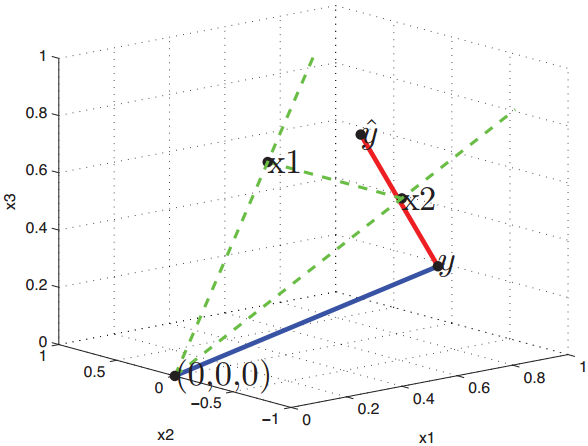
\includegraphics[scale=.50]{graphical-interpretation-of-OLS.png}
\caption{Graphical interpretation of least squares for $N=3$ examples and $D=2$ features. $\tilde{\vec{x}}_1$ and $\tilde{\vec{x}}_2$˜ are vectors in $\mathbb{R}^3$; together they define a 2D plane. $\vec{y}$ is also a vector in $\mathbb{R}^3$ but does not lie on this 2D plane. The orthogonal projection of $\vec{y}$ onto this plane is denoted $\hat{\vec{y}}$. The red line from $\vec{y}$ to $\hat{\vec{y}}$ is the residual, whose norm we want to minimize. For visual clarity, all vectors have been converted to unit norm.}
\label{fig:graphical-interpretation-of-OLS} 
\end{figure}

To minimize the norm of the residual, $\vec{y}-\hat{\vec{y}}$, we want the residual vector to be orthogonal to every column of $\vec{X}$,so˜ $\tilde{\vec{x}}_j(\vec{y}-\hat{\vec{y}})=0$ for $j=1:D$. Hence
\begin{equation}\begin{split}
\tilde{\vec{x}}_j(\vec{y}-\hat{\vec{y}})=0 & \Rightarrow \vec{X}^T(\vec{y}-\vec{X}\vec{w})=0 \\
                                           & \Rightarrow \vec{w}=(\vec{X}^T\vec{X})^{-1}\vec{X}^T\vec{y}
\end{split}\end{equation}


\subsection{SGD}
When $\mathcal{D}$ is large, use stochastic gradient descent(SGD).

\begin{align}
\because \dfrac{\partial}{\partial w_i}\text{NLL}(\vec{w})=& \sum\limits_{i=1}^N (\vec{w}^T\vec{x}_i-y_i)x_{ij} \\
\therefore w_j=& w_j - \alpha\dfrac{\partial}{\partial w_j}\text{NLL}(\vec{w}) \nonumber \\
                  =& w_j - \sum\limits_{i=1}^N \alpha(\vec{w}^T\vec{x}_i-y_i)x_{ij} \\
\therefore \vec{w}=& \vec{w}-\alpha(\vec{w}^T\vec{x}_i-y_i)\vec{x}
\end{align}


\section{Ridge regression(MAP)}
One problem with ML estimation is that it can result in overfitting. In this section, we discuss a way to ameliorate this problem by using MAP estimation with a Gaussian prior.


\subsection{Basic idea}
We can encourage the parameters to be small, thus resulting in a smoother curve, by using a zero-mean Gaussian prior:
\begin{equation}
p(\vec{w})=\prod\limits_j \mathcal{N}(w_j|0,\tau^2)
\end{equation}
where $1/\tau^2$ controls the strength of the prior. The corresponding MAP estimation problem becomes
\begin{equation}
\arg\max_{\vec{w}} \sum\limits_{i=1}^N \log{\mathcal{N}(y_i|w_0+\vec{w}^T\vec{x}_i,\sigma^2)}+\sum\limits_{j=1}^D \log{\mathcal{N}(w_j|0,\tau^2)}
\end{equation}

It is a simple exercise to show that this is equivalent to minimizing the following
\begin{equation}\label{eqn:Ridge-regression-J}
J(\vec{w})=\dfrac{1}{N}\sum\limits_{i=1}^N (y_i-(w_0+\vec{w}^T\vec{x}_i))^2+\lambda\lVert\vec{w}\rVert^2 , \lambda \triangleq \dfrac{\sigma^2}{\tau^2}
\end{equation}

Here the first term is the MSE/ NLL as usual, and the second term, $\lambda \geq 0$, is a complexity penalty. The corresponding solution is given by
\begin{equation}\label{eqn:Ridge-regression-solution}
\hat{\vec{w}}_{\mathrm{ridge}}=(\lambda\vec{I}_D+\vec{X}^T\vec{X})^{-1}\vec{X}^T\vec{y}
\end{equation}

This technique is known as \textbf{ridge regression},or \textbf{penalized least squares}. In general, adding a Gaussian prior to the parameters of a model to encourage them to be small is called $\ell_2$ \textbf{regularization} or \textbf{weight decay}. Note that the offset term $w_0$ is not regularized, since this just affects the height of the function, not its complexity.

We will consider a variety of different priors in this book. Each of these corresponds to a different form of \textbf{regularization}. This technique is very widely used to prevent overfitting.


\subsection{Numerically stable computation *}

\begin{equation}\label{eqn:Ridge-regression-SVD}
\hat{\vec{w}}_{\mathrm{ridge}}=\vec{V}(\vec{Z}^T\vec{Z}+\lambda\vec{I}_N)^{-1}\vec{Z}^T\vec{y}
\end{equation}


\subsection{Connection with PCA *}


\subsection{Regularization effects of big data}
Regularization is the most common way to avoid overfitting. However, another effective approach — which is not always available — is to use lots of data. It should be intuitively obvious that the more training data we have, the better we will be able to learn.

In domains with lots of data, simple methods can work surprisingly well (Halevy et al. 2009). However, there are still reasons to study more sophisticated learning methods, because there will always be problems for which we have little data. For example, even in such a data-rich domain as web search, as soon as we want to start personalizing the results, the amount of data available for any given user starts to look small again (relative to the complexity of the problem).


\section{Bayesian linear regression}
TODO

